\documentclass{article}
\usepackage[utf8]{inputenc}
\usepackage{listings}
\usepackage{graphicx}
\usepackage{hyperref}
\usepackage{indentfirst}
\usepackage[space=true]{accsupp}

\title{PyDesc tutorial}
\author{Tymoteusz Oleniecki }
\date{}

\lstset{    language=Python,
            frame=single,
            basicstyle=\footnotesize,
            showtabs=true,
            breaklines=true,
            breakatwhitespace=true
            }

\begin{document}

\maketitle

\section{PyDesc - general information}
    PyDesc is a Python 2.7.x library that provides classes which adapts Python environment to deal with biopolymer structures. It is designed for easy analysis of structures of both, proteins and nucleic acids, mostly using descriptors of local structure (DLS) approach (see chapter \ref{DLSsec}). Starting from very basic functionality as access to common databases of structures such as PDB, SCOP and CATH, and calculations of different geometrical features of structures or their parts, through combinations of contact criteria and calculation of contact maps, to the structural alignment of multiple structures in descriptor approach or analysis of MD trajectories -- everything makes PyDesc useful for bioinformatic tools developers and for fast data analysis for scientists.
    Basic features of library are written in Python and available to developer for expansion or modification. More advanced and computationally demanding parts are written in C and CUDA C for performance boost.
    PyDesc requires BioPython for \texttt{pdb} parsing and numpy for most calculations. Additional features are enabled with DSSP, blastp, blastn and prody installed.

\section{Basic features}
    PyDesc is able to load \texttt{pdb} files from common databases over Internet (PDB (including BioUnits), CATH, SCOP) or their local copies as well as single files from local drive. To deal with mmCIF files it loads bundle of \texttt{pdb} files in format provided by PDB.
    Loaded structures are stored in hierarchical objects, in which chains are stored in structures, mers are stored in chains and mers are simply containers for atoms and pseudoatoms useful in further analysis. It is also possible to create substructures of loaded structures such as ranges of sequential neighbours (called segments), sets of any mers or DLS (see chapter \ref{DLSsec}) for descriptor approach.
    Library provides friendly way to work with multiple structures. In case of homologous structures one can easily apply selections from one structure to another. As selection in PyDesc implements set theory approach different operations as addition or intersection of selections are easy to conduct. Dealing with non-homologous structures on the other hand is enabled thanks to modules providing alignment objects, which works on multiple alignments as well and allows to save and load files in common formats such as \texttt{FASTA}, \texttt{CSV} or \texttt{XML}.
    PyDesc provides calculation of contact maps and set of contact criteria to use for protein-protein and nucleic acid-nucleic acid interactions. It is also possible to combine provided contact criteria and to add user-defined criteria. That enables creation of DLS, which are substructures dependent on contact maps.
    Module for structural analysis, mostly written in C, provides structure comparison, (multiple) structure alignment and sequential/structural pattern fitting. Structure comparison allows for calculation of RMSD and rotation matrix using Kabsch method. It allows users to visualize superpositions (of both, pairs and multiple structures) using provided PyMOL plug-in. Calculation of structural alignment, by default, uses DLS approach and requires calculation of contact maps.
    Each of steps of structure analysis can be applied to frames of MD trajectories or states from NMR experiments.

\section{Descriptors of Local Structure -- DLS} \label{DLSsec}

    Descriptors of Local Structure (DLS) are sets of mers -- residues or nucleotides -- representing local physicochemical environment of given mer. Such substructures are useful in structure comparison and computation of alignments, but can be useful in other structural analysis.
    In approaches using DLS structures are split into smaller overlapping fragments containing central mer (residue or nucleotide) from analyzed biopolymer and all other mers that stay in contact with it. That implies the size and shape of DLS depends on used criteria of contact between mers. The better those criteria describe real interactions between chemical compounds, the more useful obtained DLSs are as approximation of local environment.
    During calculation of DLS there are two main types of contacts: short and long range. Short range contacts are assumed between mer and their sequential neighbours, so preceding and following mers are included into DLS. Long range contacts depend on applied contact criteria. While defining criteria it is necessary to decide their type (quality, e.g. combination of distance and chemical properties etc.) and their thresholds (quantity, e.g. maximal distance, maximal difference in polarity etc.; see section XXX(ccrits)). Application of such criteria to all mers gives mers that stays in contact with central mer. All short range contacts of such mers are also included as they carry a information about physicochemical context of those mers.

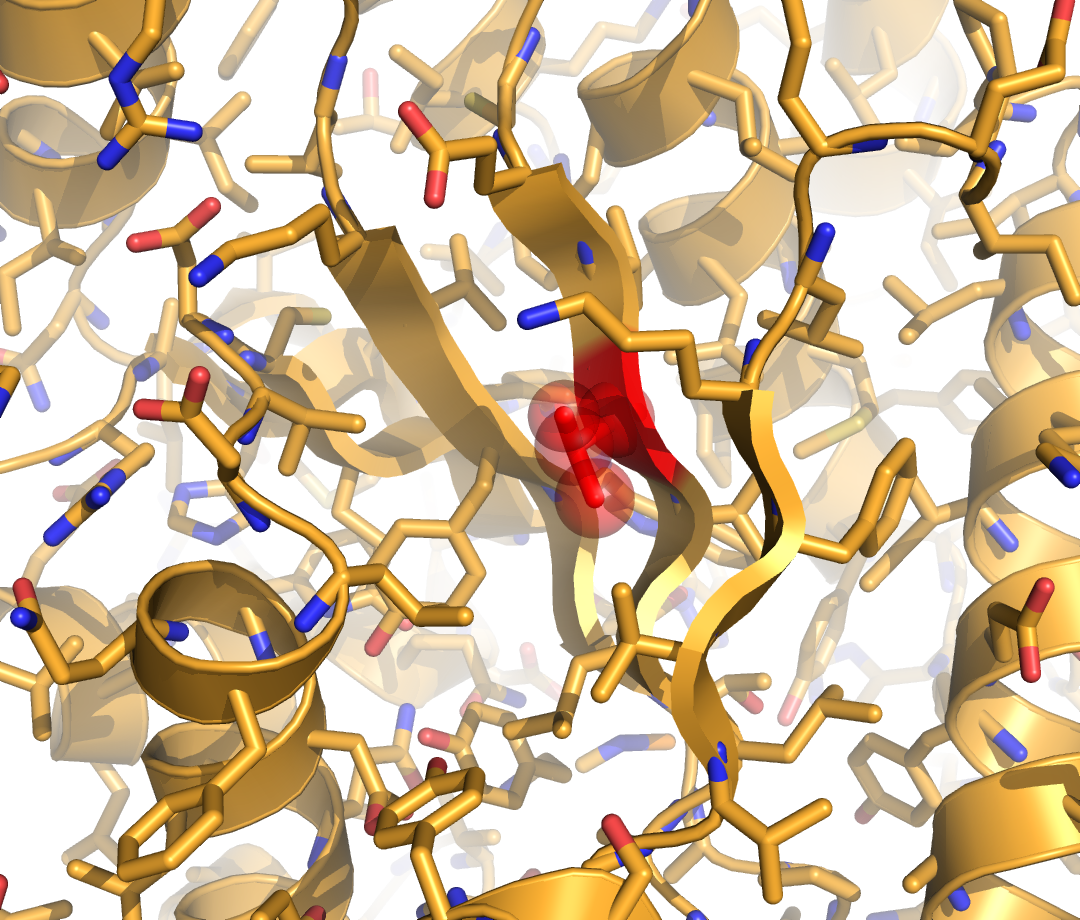
\includegraphics[width=\textwidth]{images/d1.png}
% obrazek DLS
% ew sekwencja obrazów tworzenia DLS z filmu

\section{Getting PyDesc}

    PyDesc is a library of classes written in Python 2.7. To install it, one needs Python 2.7 and dependent packages: BioPython, numpy and scipy. There are several way to download and install PyDesc:

\begin{itemize}
\item Use \texttt{git}
\begin{lstlisting}
git clone https://github.com/pawelld/PyDesc.git
\end{lstlisting}

\item Download \texttt{zip} package from \href{https://github.com/pawelld/PyDesc}{[git repository]}.

\item Use \texttt{pip} to install PyDesc from \texttt{egg} file included in repository.

\item Use easy\_{}install in downloaded directory:
\begin{lstlisting}
easy_install setup.py
\end{lstlisting}

\end{itemize}


%%%%%%%%%%%%%%%%%%%%
%SECTION -- structure loader
%%%%%%%%%%%%%%%%%%%%

\section{Getting started}

    PyDesc provides number of classes to deal with structural analysis. It can be used in development of Python scripts and programs, or as environment for fast analysis in Python interpreter. All the examples are ready to use in Python interpreter.

    To check if PyDesc library is available simply import its components in Python:
\begin{lstlisting}
import pydesc.sample
\end{lstlisting}

    Loading structures in PyDesc requires class \texttt{StructureLoader} that is a component of \texttt{structure} module:

\begin{lstlisting}
from pydesc.structure import StructureLoader
structure_loader = StructureLoader()
\end{lstlisting}

    That class provides method \texttt{load\_structure} to which user can pass reference to database entry or path to a file on local drive and get a Python list of structures from appropriate file:

\begin{lstlisting}
from pydesc.structure import StructureLoader
structure_loader = StructureLoader()
structures1 = structure_loader.load_structure("2dlc")
structures2 = structure_loader.load_structure(code="2dlc")
structures3 = structure_loader.load_structure("pdb://2dlc")
structures4 = structure_loader.load_structure("2dlc", path="my/directory/2dlc.pdb")
\end{lstlisting}

    In most cases file contains only one structure, but structures from NMR experiments or trajectories stored in \texttt{pdb} files are also able to be loaded using PyDesc.
    Structure 1 and 2 are downloaded automatically from first database to match the entry type format (\texttt{PDB} in that case). Structure 3 is loaded with forced usage of PDB. Structure 4 loads local file from \texttt{my/directory} and sets structure name to \texttt{2dlc}.
    
    That is all the basic knowledge needed to load structures. Readers interested in quick start are welcome to skip to part \ref{STCsec}. Library features behind structure loading are described below.\\

    During loader initialization User can choose what kind of database handler is to be used while loading structures. Database handler is an object responsible for connection to database. Available handlers are parts of \texttt{pydesc.dbhandler} package and are listed below:
\begin{itemize}
    \item SCOPHandler -- provides access to SCOP db.
    \item PDBHandler -- provides access to \texttt{pdb} files from PDB.
    \item PDBBundleHandler -- provides access to compatibility version of big \texttt{mmCIF} files available as bundle of \texttt{pdb} files with additional text file mapping chains.
    \item MMCIFHandler -- provides access to \texttt{mmCIF} files from PDB.
    \item CATHHandler -- provides access to CATH db.
    \item BioUnitHandler -- provides access to BioUnit part of PDB.
    \item MetaHandler -- meta handler containing all necessary handlers.
\end{itemize}

Objects of that classes can be passed to \texttt{StructureLoader} with following syntax:

\begin{lstlisting}
from pydesc.structure import StructureLoader
from pydesc.dbhandler import PDBHandler
structure_loader = StructureLoader(PDBHandler())
structure_loader = StructureLoader(handler=PDBHandler())
# both lines are equivalents
\end{lstlisting}

    By default \texttt{MetaHandler} is used.
    
    When creating a dbhandler, bear in mind that they can work in three modes:
    \begin{enumerate}
        \item Always downloading files via Internet to local cache.
        \item Always getting file from local copy of DB to local cache.
        \item Always opening files from local cache.
    \end{enumerate}

    Modes can be passed as a list to all handlers during their initialization. Subsequent modes will be executed one by one until first success or till the end of mode list, e.g.:

\begin{lstlisting}
from pydesc.structure import StructureLoader
from pydesc.dbhandler import PDBHandler
structure_loader = StructureLoader(PDBHandler(mode=[1,2,3]))
structures = structure_loader.load_structure("2DLC")
\end{lstlisting}
    
    which is equivalent to default setting, will 1) check local cache for \texttt{2dlc.pdb} file and load it if possible; otherwise it will 2) try to copy it from local DB copy to cache and load it again, but if that will end in failure, it will 3) download file from online DB to cache. Paths to local copy od DB and cache are stored in configuration manager (see chapter \ref{CONFIGsec}).

    Other argument passed to StructureLoader initializator is \texttt{parser}, which should be object with method \texttt{get\_{}structure} returning instances of structures as defined in Biopython \texttt{Bio.PDB} module. By default \texttt{MetaParser} from \texttt{pydesc.dbhandler} module is used. That object contains \texttt{PDBParser} and \texttt{mmCIFParser} from Biopyton \texttt{Bio.PDB} module, instances of both classes can be used on their own, if only passed handler returns appropriate files. E.g. one can use \texttt{PDBHandler}, which provides only \texttt{pdb} files to parser, therefore parser could be \texttt{Bio.PDB.PDBParser}.

\begin{lstlisting}
from pydesc.structure import StructureLoader
from pydesc.dbhandler import PDBHandler
from Bio.PDB import PDBParser
structure_loader = StructureLoader(handler=PDBHandler(), parser=PDBParser())
\end{lstlisting}

    When using non-default parser make sure that it can handle type of files returned by used dbhandler.

%%%%%%%%%%%%%%%%%%%%
%SECTION -- configuration
%%%%%%%%%%%%%%%%%%%%

\section{Configuration} \label{CONFIGsec}

There is a bunch of global settings influencing PyDesc library behaviour. They are all stored in \texttt{pydesc.config} module in static class \texttt{ConfigManager} with \texttt{show\_{}config} method that shows tree of configuration:

\begin{lstlisting}
import pydesc.structure
from pydesc.config import ConfigManager

ConfigManager.show_config()
\end{lstlisting}
Output:
\begin{lstlisting}
+ConfigManager
 +alignments
	-multiple_alignment_mode = strict
 +compdesc
	-ca_contact_distance = 6.0
	-force_order = 0
	-th_align_size_equiv = 3
...
\end{lstlisting}

All settings are stored in separate branches of names more or less corresponding with modules available in PyDesc. Branches containing appropriate configuration are created on module import. Settings important for certain function of library will be mentioned in appropriate chapters. Here we will present how to change and use settings using ezample of structure loaders mentioned in previous chapter.

\begin{lstlisting}
import pydesc.structure
from pydesc.config import ConfigManager

print ConfigManager.dbhandler.cachedir
\end{lstlisting}

Setting \texttt{cachedir} in \texttt{dbhandler} branch of configuration manager is a directory in which cached structure files are stored. Lets assume that User conducts an experiment on set of structures. At some point he decides to test some other parameters in new directory, and wants to run modified scripts on the same set of structures. To avoid downloading and caching the same structures in new directory, User adds the following line:
\begin{lstlisting}
ConfigManager.dbhandler.cachedir = '../old/directory/biodb/'
# equivalent:
ConfigManager.dbhandler.cachedir.set('../old/directory/biodb/')
\end{lstlisting}


%%%%%%%%%%%%%%%%%%%%
%SECTION -- structures
%%%%%%%%%%%%%%%%%%%%

\section{Dealing with structures} \label{STCsec}

Let us assume that one has already loaded a structure:

\begin{lstlisting}
from pydesc.structure import StructureLoader
structure_loader = StructureLoader()
structures = structure_loader.load_structure("2dlc")
structure = structures[0]
\end{lstlisting}

    As doing so in Python interpreter every time just to test some simple commands is arduous, for the sake of tuition PyDesc provides \texttt{get} function in \texttt{sample} module, which can be used instead.

\begin{lstlisting}
from pydesc.sample import get
structure = get("2dlc")
\end{lstlisting}
    
    That function returns only one structure from list of loaded structures. By default it is the first one, but User can pass index of structure to be returned as second argument. Note that lists in Python are indexed from 0.

%
%
%
\subsection{Getting mers and substructures}

    PyDesc structures and substructures consist of mers (residue, nucleotide, ligands or ions), which consist of atoms. Each entity is represented by separate iterable object, so one way to get to building blocks of any level is to loop over their elements:

\begin{lstlisting}
for mer in structure:
    print mer
    for atom in mer:
        print atom
\end{lstlisting}
Output:
\begin{lstlisting}
<Residue: GLN no. 1, PDB: A6>
<Atom C  : 18.040001 6.891000 -2.685000>
<Atom CA : 16.721001 7.525000 -3.144000>
<Atom CB : 15.546000 6.793000 -2.485000>
<Atom CD : 13.952000 4.840000 -2.513000>
<Atom CG : 15.147000 5.500000 -3.170000>
<Atom N  : 16.635000 7.521000 -4.591000>
<Atom NE2: 14.089000 3.561000 -2.181000>
<Atom O  : 18.969000 6.780000 -3.474000>
<Atom OE1: 12.928000 5.490000 -2.312000>
<Pseudoatom : 16.721001 7.525000 -3.144000>
<Pseudoatom cbx: 14.779633 6.315571 -2.055182>
<Pseudoatom rc: 15.780779 6.100111 -2.950556>
\end{lstlisting}

Often we are not interested in whole structure, but in only one chain of it. Objects representing chains are created automatically and are stored in \texttt{chains} attribute of \texttt{Structure} instance. Class \texttt{Structure} also provides \texttt{get\_chain} method, which takes chain name as \texttt{str}:

\begin{lstlisting}
print structure.chains
print structure.get_chain('X')
\end{lstlisting}
Output:
\begin{lstlisting}
[<Chain 2dlcY>, <Chain 2dlcX>]
<Chain 2dlcX>
\end{lstlisting}

Sample structure \texttt{2DLC} consists of chains "X" and "Y".

Chains in PyDesc are very similar to whole structures and any other part of structure we will deal with in that tutorial. All of them provide method for getting their mers using Python syntax, which behaves slightly different than its equivalent for python sequential types:

\begin{lstlisting}
chainX = structure.get_chain('X')
print structure[0], structure[0].ind
print structure[1], structure[1].ind
print chainX[0], chainX[0].ind
print chainX[75], chainX[75].ind
\end{lstlisting}
Output:
\begin{lstlisting}
<Nucleotide:   C no. 1, PDB: Y501> 1
<Nucleotide:   C no. 1, PDB: Y501> 1
<Residue: ASP no. 75, PDB: X8> 75
<Residue: ASP no. 75, PDB: X8> 75
\end{lstlisting}

Mers in PyDesc are indexed from 1. Index 0 always returns first mer of the (sub)structure. PyDesc mer id, stored in \texttt{ind} attribute of mer, is created once at the creation of structure the mer belongs to and identifies mer in that particular \textbf{structure}, thus picking chain from the middle of the structure leads to shifted indexing. Attempts to pick mer of index not occurring in (sub)structure leads to \texttt{IndexError}. This is very useful in some cases but can be confusing for new Users. In above example chain X starts with mer 75. If one wants to index elements of PyDesc structure as in Python, simply convert PyDesc structure to Python sequential type, e.g. list or tuple:

\begin{lstlisting}
print tuple(chainX)[0], list(chainX)[1]
\end{lstlisting}
Output:
\begin{lstlisting}
<Residue: ASP no. 75, PDB: X8> <Residue: PRO no. 76, PDB: X9>
\end{lstlisting}

Users are allowed to get parts or slices of structures:

\begin{lstlisting}
seg = structure[75: 82]
for mer in seg: print mer
\end{lstlisting}

Note that mer 82 is a part of returned \texttt{Segment} instance! That is another difference between PyDesc and Python sequential types indexing. That means that expressions:

\begin{lstlisting}
seg1 = structure[75: 75]
mer75 = structure[75]
\end{lstlisting}

return different type of objects. First one returns \texttt{Segment} instance of length 1, containing only 75th mer. Second one returns mer itself, residue in that case.

Structures can be easily joined using \texttt{+} operator:

\begin{lstlisting}
mix = structure[75: 82] + structure[84:85] + structure[90:90]
\end{lstlisting}

This kind of substructures are instances of \texttt{UserStructure} objects and has all the methods already presented here for \texttt{Chain}, \texttt{Segment}, \texttt{Structure} classes. Note that adding single mer to substructure requires adding 1-mer length segment ($structure[90:90]$). Attempt to add mer ($structure[90]$) will end up in \texttt{AttributeError}.

%
%
%
\subsection{Getting atoms and pseudoatoms}

Mers are sets of atoms and pseudoatoms (like geometrical center of side chain). Iteration over mer instance gives subsequent atoms and pseudoatoms:

\begin{lstlisting}
for atom in structure[90]:
    print atom
\end{lstlisting}
Output:
\begin{lstlisting}
<Atom C  : -2.385000 36.616001 173.134995>
<Atom CA : -2.743000 37.533001 171.970001>
<Atom CB : -3.075000 38.953999 172.513000>
<Atom CG1: -1.882000 39.539001 173.264999>
<Atom CG2: -3.498000 39.891998 171.386993>
<Atom N  : -3.867000 36.938000 171.257996>
<Atom O  : -3.216000 36.372002 174.016998>
<Pseudoatom : -2.813667 36.223667 171.880325>
<Pseudoatom cbx: -3.288228 39.866638 172.861740>
<Pseudoatom rc: -2.952286 37.977715 172.506424>
\end{lstlisting}

To get certain atom, one can use syntax similar to one used in Python dictionaries:
\begin{lstlisting}
structure[90]['CA']
\end{lstlisting}
It works also for pseudoatoms, which usually are also an attribute of mer:
\begin{lstlisting}
structure[90]['cbx']
structure[90].cbx
\end{lstlisting}

\texttt{cbx} is a pseudoatom defined for residues used by PyDesc default contact definition. It is vector $<{\rm C_{\alpha{}}}, {\rm C_{\beta{}}}>$ extended by 1 \AA{}.


There are also alternative iterators for mer, available using mer methods:
\begin{itemize}
    \item \texttt{\_\_iter\_\_} -- default, iterating over all atoms and pseudoatoms.
    \item \texttt{iter\_{}atoms} -- iterating over atoms only.
    \item \texttt{iter\_{}atomsbb} -- iterating over backbone atoms only.
    \item \texttt{iter\_{}atomsnbb} -- iterating over non-backbone atoms only.
\end{itemize}

Distinguish of backbone and non-backbone atoms bases on setting \texttt{backbone\_{}atoms} in branch \texttt{ConfigManager.monomer.*}, where asterisk is to be replaced with name of chainable mer, basically \texttt{residue} or \texttt{nucleotide}. Configuration stores any sequential type containing names of atoms as strings (with no spaces). E.g.:
\begin{lstlisting}
from pydesc.config import monomer
from pydesc.config import ConfigManager

print ConfigManager.monomer.residue.backbone_atoms 
\end{lstlisting}
Output:
\begin{lstlisting}
('N', 'CA', 'C')
\end{lstlisting}

%
%
%
\subsection{DLS, Contacts, Elements}

There is also special kind of substructures containing parts of structure that are not sequential neighbours: DLSs (see chapter \ref{DLSsec}). That kind of structures depend on contact maps, which are matter of next chapter (\ref{CMAPsec}), here we will use default settings to calculate them.

To create DLS one needs to provide \texttt{Element} subclass instance (\texttt{ElementChainable}, \texttt{ElementOther}) of central mer and elements of all mers that stay in contact with central mer. Element chainable is special kind of \texttt{Segment} of odd number of mers with distinguished central mer. By default elements are segments of length 5 and depends on setting \texttt{pydesc.config.ConfigManager.element.element\_{}chainable\_{}length}.
Elements of mers in contact with central mer should delivered as attributes of \texttt{Contact} instances, so second object needed to form a DLS is list of contacts.
All classes, \texttt{Element} adn subclasses, \texttt{Contact} , as well as \texttt{ProteinDescriptor} or \texttt{NucleotideDescriptor} can be imported from \texttt{pydesc.structure} module.

Assuming that one knows the list of PyDesc indexes of mers that stays in contact with certain mer (list \texttt{cnt1} in example below), lets say 90 in \texttt{2DLC}, creation of descriptor goes as follow:

\begin{lstlisting}
cnt1 = [84, 87, 93, 96, 280, 281, 282]

from pydesc.structure import ElementChainable
from pydesc.structure import Contact
from pydesc.structure import ProteinDescriptor

element90 = ElementChainable(structure[90])
descriptor90 = ProteinDescriptor(element90, [Contact(ElementChainable(structure[i]), element90) for i in cnt1])
\end{lstlisting}

Contacts could be read from contact map calculated with PyDesc module.

Similarly to this, one could create a nucleotide descriptor using \texttt{NucleotideDescriptor} class with appropriate element and contacts list. As that procedure is complicated and could be executed very often, each subclass of \texttt{AbstractDescriptor} provide static method of descriptor building basing on contact map calculated for structure from which mer comes from:

\begin{lstlisting}
from pydesc.structure import StructureLoader
from pydesc.structure import Element
from pydesc.structure import ProteinDescriptor

structure = StructureLoader().load_structure('2dlc')[0]
structure.set_contact_map()

element90 = Element(structure[90])
descriptor90 = ProteinDescriptor.build(element90)
\end{lstlisting}

It is also possible to pass other contact map to that method as second argument. For structures containing both, protein and nucleic acids, it may be convenient to use method \texttt{build} provided by \texttt{AbstractDescriptor} class, which takes element and decides what type of descriptor to build:

\begin{lstlisting}
from pydesc.structure import StructureLoader
from pydesc.structure import Element
from pydesc.structure import AbstractDescriptor

structure = StructureLoader().load_structure('2dlc')[0]
structure.set_contact_map()

element90 = Element.build(structure[90])  #residue
descriptor90 = AbstractDescriptor.build(element90)

element20 = Element.build(structure[25])  #nucleotide
descriptor20 = AbstractDescriptor.build(element20)

print descriptor90
print descriptor20
\end{lstlisting}
Output:
\begin{lstlisting}
<ProteinDescriptor of 2dlc:X23>
<NucleotideDescriptor of 2dlc:Y526>
\end{lstlisting}

Often it is necessary to create all possible DLSs for given structure, which can be easily done with \texttt{create\_{}descriptors} static method, which returns generator for subsequent DLSs:

\begin{lstlisting}
from pydesc.structure import StructureLoader
from pydesc.structure import AstractDescriptor

structure = StructureLoader().load_structure('2dlc')[0]
structure.set_contact_map()
DLSgen = AbstractDescriptor.create_descriptors(structure)
DLSs = list(DLSgen)
\end{lstlisting}

For mers, for which DLS cannot be created \texttt{None} is returned. That allows for convenient usage of \texttt{zip} function on result:

\begin{lstlisting}
DLSgen = AbstractDescriptor.create_descriptors(structure)
for mer, its_DLS in zip(structure, DLSgen):
    print mer, its_DLS
\end{lstlisting}
Output:
\begin{lstlisting}
<Nucleotide:   C no. 1, PDB: Y501> None
<Nucleotide:   U no. 2, PDB: Y502> None
<Nucleotide:   C no. 3, PDB: Y503> <NucleotideDescriptor of 2dlc:Y503>
<Nucleotide:   U no. 4, PDB: Y504> <NucleotideDescriptor of 2dlc:Y504>
<Nucleotide:   C no. 5, PDB: Y505> <NucleotideDescriptor of 2dlc:Y505>
<Nucleotide:   G no. 6, PDB: Y506> <NucleotideDescriptor of 2dlc:Y506>
...
\end{lstlisting}


%%%%%%%%%%%%%%%%%%%%
%SECTION -- selections
%%%%%%%%%%%%%%%%%%%%

\section{Selections} \label{SELEsec}

Selections are classes that allows users to apply set theory operations to structures and substructures. In other words -- thanks to \texttt{selection} module it is possible to use structures as sets of mers, which they are. What is more -- it allows to generalize operations on structures with consistent PDB numbering. Lets see how it works. There are two crystals of amicyjanins with different asymmetric units: \texttt{1sfd} and \texttt{2gb1}:

\begin{lstlisting}
from pydesc.structure import StructureLoader

stc_1sfd = StructureLoader().load_structure('1sfd')[0]
stc_2gb1 = StructureLoader().load_structure('2gb1')[0]
\end{lstlisting}

Proteins are mutated, therefore they differ in positions 52 and 94. What is more -- \texttt{1sfd} consists of two chains. Let us pick the whole loop and $\beta$-strand containing mutated residue 94 in \texttt{1sfd}:

\begin{lstlisting}
from pydesc.selection import Range

sele = Range('A92', 'A96', distinguish_chains=False)
\end{lstlisting}

We can also get it using method of \texttt{Segment} class:

\begin{lstlisting}
sele = stc1['A92':'A96'].select(distinguish_chains=False)
\end{lstlisting}

What is the difference between \texttt{Range} and \texttt{Segment} then? Selection object does not store any structural data, only information that selected mers are between IDs 92 and 96 (in chain A if argument \texttt{distinguish\_{}chains} was set to True). It can be applied to any structure and used to get substructure or to create new independent structure basing on the old one:

\begin{lstlisting}
loop1sfdA = sele.select(stc_1sfd.get_chain('A'))
loop1sfdB = sele.select(stc_1sfd.get_chain('B'))
loops1sfd = sele.select(stc_1sfd)
loop2gb1 = sele.select(stc_2gb1)
\end{lstlisting}

\texttt{Range} is probably the most useful selection, but most basic is \texttt{Set}. It takes list of residue IDs and can be useful in cases where we deal with structures consisting of mers with insertion codes. To convert range selection to set selection one needs to give a structure on which that conversion is to be made:

\begin{lstlisting}
seleSet = sele.specify(stc_1sfd)
\end{lstlisting}

In range defined in \texttt{sele} in structure \texttt{stc\_{}1sfd} there are no residues with insertion codes. But one may want to apply that selection to other structure. Applying a range selection will embrace all residues, while applying set selection obtained from range selection will pick only residues of IDs present in structure that was used as base to set creation.

All kinds of selections are listed below, with arguments demanded by initializator and respective class that returns that kind of selection upon call of its \texttt{select} method:

\begin{itemize}
    \item Set, list of PDB IDs (\texttt{str}), \texttt{UserStructure}, \texttt{Monomer}
    \item Range, starting and ending PDB IDs (\texttt{str}), \texttt{Segment}
    \item ChainSelection, chain name (\texttt{str}), \texttt{Chain}
    \item MonomerName, PDB residue name (\texttt{str}), \texttt{Segment}
    \item MonomerType, \texttt{Monomer} subclass, --
    \item Everything, --, \texttt{Structure}
    \item Nothing, --, --
\end{itemize}

Basic operation known from set theory are provided:

\begin{lstlisting}
from pydesc.selection import Everything
from pydesc.selection import MonomerType
from pydesc.selection import MonomerName
from pydesc.selection import ChainSelection

sele1 = MonomerName('TYR')      # selecting all tyrosines
sele2 = Everything() - sele1    # everything but tyrosines
sele3 = ChainSelection('A')     # chain A
sele4 = sele3 * sele2           # chain A except tyrosines
\end{lstlisting}

%%%%%%%%%%%%%%%%%%%%
%SECTION -- contact maps
%%%%%%%%%%%%%%%%%%%%

\section{Contact maps} \label{CMAPsec}

\subsection{Basics, default criteria}

Contact map contains information about contacts between mers in structure. To create one, one needs to know criteria of contact. First let us look at contact maps with default PyDesc criteria. PyDesc provides methods for checking values, getting contacts and saving all non-zero values in \texttt{CSV} file:
\begin{lstlisting}
from pydesc.structure import StructureLoader

structure = StructureLoader().load_structure('2dlc')[0]
structure.set_contact_map()

print structure.contact_map
with open("2dlc_cmap.csv", "w") as fhobj:
    structure.contact_map.dump(fhobj)

print structure.contact_map.get_monomer_contacts(90)

print structure.contact_map.get_contact_value(90, 50)
print structure.contact_map.get_contact_value(90, 96)
print structure.contact_map.get_contact_value(90, 281)
\end{lstlisting}
Output:
\begin{lstlisting}
[(90, 96, 1), (90, 281, 2), (90, 84, 2), (90, 87, 2), (90, 280, 1), (90, 89, 2), (90, 282, 1), (90, 91, 2), (90, 92, 1), (90, 93, 2)]
0
1
2
\end{lstlisting}


Data stored in contact map can be passed to any file-like object including streams and files. It calls \texttt{write} method on passed object and feeds it with string containing as manly lines, as many contacts there is in structure (times two, as they are assumed to be symmetrical), in each line placing two PDB ids and $value$ that can be 1 or 2.

As contact criteria in PyDesc uses tree-value logic the latter mean reliable contact, and the former -- possible contact. Zero denote no contact. Criterion usually consist of some quality requirements (what features of mer should be taken into account) and quality requirements (threshold, below which criterion is satisfied). By default PyDesc uses:
\begin{itemize}
    \item for residues of indexes $i$ and $j$:
    $$distance(C_{\alpha{}, i}, C_{\alpha{}, j}) \leq 6.00 \pm 0.50 \textrm{\AA}$$
    OR
    $$distance(C_{\beta{}x, i}, C_{\beta{}x, j}) \leq 6.50 \pm 0.50 \textrm{\AA}$$
    $$\land$$
    $$distance(C_{\beta{}x, i}, C_{\beta{}x, j}) - distance(C_{\alpha{}, i}, C_{\alpha{}, j}) \leq 0.75 \pm 0.00 \textrm{\AA}$$
    where:\\
    $C_{\alpha{}, a}$ -- coordinates of alpha carbon of $a$-th residue,\\
    $C_{\beta{}x, a}$ -- coordinates of extended beta carbon of $a$-th residue.
    \item for nucleotides of indexes $i$ and $j$:
    $$distance(R_{c, i}, R_{c, j}) \leq 6.25 \pm 0.00 \textrm{\AA}$$
    OR
    $$distance(R_{c, i}, I) \leq 7.40 \pm 0.00 \textrm{\AA} \land{} distance(R_{c, j}, I) \leq 7.40 \pm 0.00 \textrm{\AA}$$
    where:\\
    $R_{c, a}$ -- $a$-th nucleotide ring center,\\
    $I$ -- ion coordinates.
\end{itemize}

Standard error notation was used here to indicate range in which contacts get value of 1.

%
%simple and combined criteria
%
\subsection{Simple and combined pre-defined criteria}

All pre-defined contact criteria and abstract classes are implemented in \texttt{contacts} module. For example first part of default criterion for residues measures distance of their alpha carbons and checks if it is under the threshold. It could be used alone for contact map calculation:

\begin{lstlisting}
from pydesc.structure import StructureLoader
from pydesc.contacts import CaContact

structure = StructureLoader().load_structure('2dlc')[0]
structure.set_contact_map(CaContact())
print structure.contact_map.get_monomer_contacts(90)
\end{lstlisting}
Output:
\begin{lstlisting}
[(90, 281, 2), (90, 280, 1), (90, 89, 2), (90, 282, 1), (90, 91, 2), (90, 92, 1), (90, 93, 1)]
\end{lstlisting}

Note that with such criterion there is no contacts between any nucleotides (residues 1-74 for \texttt{2DLC}).

By default that criterion uses threshold equals to 6.00 and so called \textit{undecidable range} of 0.50, which can be changed simply by passing them to criterion object initializator:

\begin{lstlisting}
structure.set_contact_map(CaContact(8., .75))
print structure.contact_map.get_monomer_contacts(90)
\end{lstlisting}
Output:
\begin{lstlisting}
[(90, 279, 1), (90, 281, 2), (90, 280, 2), (90, 84, 2), (90, 87, 1), (90, 88, 2), (90, 89, 2), (90, 282, 2), (90, 91, 2), (90, 92, 2), (90, 93, 2)]
\end{lstlisting}

If no arguments is passed to initializator, settings from configuration manager:

\begin{lstlisting}
structure.set_contact_map(CaContact())
print structure.contact_map.get_monomer_contacts(90)
ConfigManager.contacts.ca_contact_distance = 8.0
ConfigManager.contacts.ca_contact_undecidable_range = 0.75
structure.set_contact_map(CaContact())
print structure.contact_map.get_monomer_contacts(90)
\end{lstlisting}
Output:
\begin{lstlisting}
[(90, 281, 2), (90, 280, 1), (90, 89, 2), (90, 282, 1), (90, 91, 2), (90, 92, 1), (90, 93, 1)]
[(90, 279, 1), (90, 281, 2), (90, 280, 2), (90, 84, 2), (90, 87, 1), (90, 88, 2), (90, 89, 2), (90, 282, 2), (90, 91, 2), (90, 92, 2), (90, 93, 2)]
\end{lstlisting}

Difference between calling initializator with arguments and changing default settings is in behaviour of already existing contact criterion:

\begin{lstlisting}
ConfigManager.contacts.ca_contact_distance = 8.0
ConfigManager.contacts.ca_contact_undecidable_range = 0.75
ca_crit_SD = CaContact()
ca_crit_8_75 = CaContact(8., .75)

structure.set_contact_map(ca_crit_SD)
print structure.contact_map.get_monomer_contacts(90)
structure.set_contact_map(ca_crit_8_75)
print structure.contact_map.get_monomer_contacts(90)
\end{lstlisting}
Output:
\begin{lstlisting}
[(90, 279, 1), (90, 281, 2), (90, 280, 2), (90, 84, 2), (90, 87, 1), (90, 88, 2), (90, 89, 2), (90, 282, 2), (90, 91, 2), (90, 92, 2), (90, 93, 2)]
[(90, 279, 1), (90, 281, 2), (90, 280, 2), (90, 84, 2), (90, 87, 1), (90, 88, 2), (90, 89, 2), (90, 282, 2), (90, 91, 2), (90, 92, 2), (90, 93, 2)]
\end{lstlisting}

Result is the same, but in case of any change in settings:

\begin{lstlisting}
ConfigManager.contacts.ca_contact_distance = 6.0
ConfigManager.contacts.ca_contact_undecidable_range = 0.50

structure.set_contact_map(ca_crit_SD)
print structure.contact_map.get_monomer_contacts(90)
structure.set_contact_map(ca_crit_8_75)
print structure.contact_map.get_monomer_contacts(90)
\end{lstlisting}
Output:
\begin{lstlisting}
[(90, 279, 1), (90, 281, 2), (90, 280, 2), (90, 84, 2), (90, 87, 1), (90, 88, 2), (90, 89, 2), (90, 282, 2), (90, 91, 2), (90, 92, 2), (90, 93, 2)]
[(90, 279, 1), (90, 281, 2), (90, 280, 2), (90, 84, 2), (90, 87, 1), (90, 88, 2), (90, 89, 2), (90, 282, 2), (90, 91, 2), (90, 92, 2), (90, 93, 2)]
\end{lstlisting}

the \texttt{ca\_crit\_SD} will change values on the fly.

Second part of default criterion is a combined criterion, first part of which is basically the same as previously described \texttt{CaContct}, just calculating distance between \texttt{cbx} with different threshold. For that purpose there is another class \texttt{CbxContact} in appropriate module. One could be interested in criterion a bit easier than default one: alternative of \texttt{ca} i \texttt{cbx} criteria. With class \texttt{ContactsAlternative} it is as simple as:

\begin{lstlisting}
from pydesc.contacts import ContactsAlternative
from pydesc.contacts import CaContact
from pydesc.contacts import CbxContact

ccrit = ContactsAlternative(CaContact(), CbxContact())
\end{lstlisting}

One can pass as many contact criteria as needed. PyDesc delivers also \texttt{ContactsConjunction} and \texttt{ContactExclusiveDisjunction} classes, which can also be called with Python operators:

\begin{lstlisting}
from pydesc.contacts import CaContact
from pydesc.contacts import CbxContact

alt = CaContact() | CbxContact()  #alternative
con = CaContact() & CbxContact()  #conjunction
exd = CaContact() ^ CbxContact()  #exclusive disjuntion
\end{lstlisting}

It is also possible to easily enerate negative criteria with \texttt{Not} class decorator, which for combined criteria reqires a bit tricky syntax:

\begin{lstlisting}
from pydesc.contacts import ContactsAlternative
from pydesc.contacts import CaContact
from pydesc.contacts import CbxContact

n_Ca = Not(CaContact)()
n_alt = Not(ContactsAlternative)(CaContact(), CbxContact())
\end{lstlisting}

%
% own simple criteria
%
\subsection{Defining own simple criteria}

In most cases it is sufficient to use pre-defined classes of criteria. PyDesc provides following \textbf{abstract} (one should not create instance of those classes, only create classes that inherit from them) classes:
\begin{itemize}
    \item \texttt{ContactCriterion} -- generic criterion.
    \item \texttt{PointsDistanceCriterion} -- criteria basing on distance between (pseudo)atoms of choice.
    \item \texttt{SetDistanceCriterion} -- criteria based on set of distances between more than two pairs of atoms from different mers.
    \item \texttt{VectorDistanceCriterion} -- criteria based on orientation of vectors distinguished in mers.
    \item \texttt{DihedralAngleCriterion} -- criteria based on dihedral angels between planes spanned on mer atoms.
\end{itemize}

\texttt{PointsDistanceCriterion} is the class of most widely used type of geometrical criteria. Extending this class is the best way to get own criteria dependent on distance between (pseudo)atom of choice. For example, lets define criterion for side chain geometrical center, which is stored in \texttt{rc} attribute of any chainable mer (for sake of example, as that criterion is implemented in \texttt{RcContact} class):

\begin{lstlisting}
from pydesc.contacts import PointsDistanceCriterion

class RcCrt(PointsDistanceCriterion):
    monomer_hallmark = 'rc'

crt = RcCrt(4., 1.)
\end{lstlisting}

It requires only static attribute \texttt{monomer\_{}hallmark} set to string containing name of attribute to be used in distance calculation. Of course, that is more likely to be useful for types of mers defined by Users, with their own pseudoatoms.

If no arguments will be passed to initializator -- class will automatically seek for settings in configuration manager in \texttt{pydesc.config.ConfigManager.contacts} branch. One important setting is \texttt{*attribute*\_contact\_distance}, and second -- \texttt{*attribute*\_contact\_undecidable\_range}, where \textit{*attribute*} will be replaced by class \texttt{monomer\_{}hallmark} attribute.

Similarly for \texttt{SetDistanceCriterion} one needs to define names of mers attributes that are lists or dicts of atoms to be searched for:

\begin{lstlisting}
from pydesc.contacts import PointsDistanceCriterion

class PaACrt(SetDistanceCriterion):
    monomer_hallmark = 'pseudoatoms'
    monomer_hallmark2 = 'atoms'

crt = PaACrt(criterion_distance=4.5, undecidable_range=.5, num_of_checked_pairs=2)
\end{lstlisting}

Initializator of such criteria can be feed with threshold and undecidable range, but also with number of pairs to meet those criteria. By default it is set to 2.

%
% own criteria with is_in_contact methdo
%
\subsection{Defining own mers, pseudoatoms and contact criteria}

By deafult PyDeck works on all-atom representation and is meant to be a tool in protein and nucleic acid structures analysis, but can be also used for other representations and for other molecules. In both cases it is more convenient to define new kinds of mers. Mers in PyDesc are stored in \texttt{pydesc.monomer} module. Main class, \texttt{Monomer} is abstract and has two subclasses: \texttt{MonomerChainable} and \texttt{MonomerOther}, first of which is, again, an abstract superclass for \texttt{Nucleotide} and \texttt{Residue} classes, while later is superclass for \texttt{Ligand} and \texttt{Ion}. Lets assume we have some \texttt{pdb} file containing protein structure, but in representation containing only carbons alpha, beta and some pseudoatoms representing side chain, called \textit{SSn}, where $n$ is number of that pseudoatom (e.g. MARTINI representation). As that representation lacks important backbone atoms -- by default PyDesc would fail to load it, unless new subclass of \texttt{MonomerChainable} is defined. We will be interesed in, lets say, contact map of that protein with contact criterion defined as distance between \textit{SS1} pseudoatoms, but only for serines. Therefore we need:

\begin{lstlisting}
from pydesc.monomer import MonomerChainable
from pydesc.monomer import Monomer

class ReducedResidue(MonomerChainable):
    def __init__(self, pdb_residue, structure_obj, **kwargs):
        Monomer.__init__(self, pdb_residue, structure_obj, **kwargs)
    @property
    def ss1(self):
        return self.atoms['SS1']
\end{lstlisting}

As you can notice, this class simply calls \texttt{Monomer} initializator (instead of \texttt{MonomerChainable} to avoid questions about backbone atoms) and defines a new property, \texttt{ss1}, which returns \textbf{atom} called \textit{SS1}. In PyDesc everything that is read from \texttt{pdb} file is atom and to make it accessible for contact criteria -- one needs to define a property returning that atom.

Now movin og to contact criteria. As mentioned before, Users criterion contact should be subclass of classes provided in \texttt{pydesc.contacts} module. Usually contact criteria are classes that use two methods to tell if two mers are in contact or not: \texttt{\_{}calculate\_{}distance} and \texttt{\_{}is\_{}in\_{}contact}. Both should take two mer instances as arguments. First one returns distance or array of distances, dependent on criterion type. Second one should call first one and compare results obtained for given mers with thresholds. For this case we should write:

\begin{lstlisting}
from pydesc.contacts import ContactCriterion

class SerSS1Crt(ContactCriterion):
    def __init__(self, threshold, undecidable_range):
        self.thr = threshold
        self.undr = undecidable_range

    def _calculate_distance(self, m1, m2, **kwargs):
        return (m1.ss1 - m2.ss2).calculate_length()

    def _is_in_contact(self, m1, m2, **kwargs):
        if m1.name != m2.name != 'SER':
            return 0
        dist = self._calculate_distance(m1, m2)
        if dist < self.thr - self.undr:
            return 2
        elif dist < self.thr + self.undr:
            return 1
        return 0
\end{lstlisting}

With both those classes we are ready to load file with such reduced representation and calculate contact map for criterion concerning \textit{SS1} pseudoatoms in serines only. Structure in that representation is provided as \texttt{IOStream} (file-like object) within \texttt{pydesc.sample} module as result of \texttt{get\_{}MARTINI\_{}structure}, so to test it use:


\begin{lstlisting}
from pydesc.sample import get_MARTINI_structure

s = get_MARTINI_structure()
s.set_contact_map(SerSS1Crt(5.0, 0.5))
\end{lstlisting}

%%%%%%%%%%%%%%%%%%%%
%SECTION -- Descriptors of local structure
%%%%%%%%%%%%%%%%%%%%

\section{DLS: descriptors of local structure} \label{PyDLSsec}

That chapter will describe advanced usage of descriptors and is under construction.


%%%%%%%%%%%%%%%%%%%%
%SECTION -- cydesc
%%%%%%%%%%%%%%%%%%%%

\section{Structure comparison} \label{CyDESCsec}

Every module presented so far is written in Python, therefore is easy to modify and extend. As structure comparison is computationally demanding, to speed up process -- parts responsible for that feature in PyDesc are written in \texttt{C} and not available for modifications.

All modules are availible in \texttt{pydesc.cydesc} subpackage. There are three main modules: \texttt{overfit} for calculation of superposition of already aligned structures, \texttt{fitdesc} for finding patterns in structures and \texttt{compdesc} for descriptor comparison.

%
% overfit
%
\subsection{OverFit}

Module for structure superposition calculation.
Lets show how it works on an example: in aminoacyl-tRNA structure Rossmann fold is present.
Corresponding substructures in \texttt{1n3l}, residues A181-A212 and \texttt{2dlc}, residues X285-X216 slightly differ in sequence, but show high similarity in structure. To calculate RMSD and rotation matrix for their superposistion with PyDesc simply write:

\begin{lstlisting}
from pydesc.structure import StructureLoader
from pydesc.cydesc.overfit import Overfit

stc_1n3l = StructureLoader().load_structure('1n3l')[0]
stc_2dlc = StructureLoader().load_structure('2dlc')[0]

ovf = Overfit()
ovf.add_structure(stc_1n3l['A181': 'A212'], stc_2dlc['X185': 'X216'])
results = ovf.overfit()

print results
\end{lstlisting}
Output:
\begin{lstlisting}
(0.47124961018562317, <pydesc.geometry.TRTMatrix object at 0x7f4ab52eda90>)
\end{lstlisting}

Method \texttt{overfit} returns tuple of two objects: floating number, which is RMSD and PyDesc \texttt{TRTMatrix}, which can be applied to transform objects. Using this matrix to transform \texttt{1n3l} will superimpose it to \texttt{2dlc}:

\begin{lstlisting}
stc_1n3l.trt_matrix = stc_1n3l.trt_matrix.combine(results[1])
\end{lstlisting}

Comarping multiple structures is possible thanks to \texttt{Multifit} object, for which principles are the same:

\begin{lstlisting}
stc_5thl = StructureLoader().load_structure('5thl')[0]

mft = Multifit()
mft.add_structure(stc_1n3l['A181': 'A212'], stc_2dlc['X185': 'X216'], stc_5thl['A181': 'A212'])
results = mft.multifit()
\end{lstlisting}

Except that for this object result is a list of pairs: RMST and rotation matrix, that could be applied to subsequent objects passed to \texttt{add\_{}structure} method.

The whole procedure can be shorten by simple call of function \texttt{overfit} from that module:

\begin{lstlisting}
from pydesc.cydesc.overfit import overfit

results = overfit(stc_1n3l['A181': 'A212'], stc_2dlc['X185': 'X216'])
\end{lstlisting}

The same works for \texttt{multifit} function.

%
% compdesc
%
\subsection{CompDesc}

Compdesc is used to compare descriptors defined as in chapter \ref{DLSsec} and obtaines as described in chapter \ref{PyDLSsec}. For two structures loaded in previous example, lets compare all possible descriptors. First we create them:

\begin{lstlisting}
from pydesc.structure import ProteinDescriptor
from pydesc.cydesc.compdesc import CompDesc

stc_1n3l.set_contact_map()
stc_2dlc.set_contact_map()

dscs_1n3l = [i for i in ProteinDescriptor.create_descriptors(stc_1n3l) if isinstance(i, ProteinDescriptor)]
dscs_2dlc = [i for i in ProteinDescriptor.create_descriptors(stc_2dlc) if isinstance(i, ProteinDescriptor)]

results = []
for i in dscs_1n3l:
    row = []
    for j in dscs_2dlc:
        row.append(CompDesc(i, j).compdesc())
\end{lstlisting}

Each results contains three elements: RMAS, pair alignment object (see chapter \ref{ALGsec}) and rotation matrix, as it was in case of overfit.

%
% fitdesc
%
\subsection{FitDesc}

\texttt{FitDesc} from \texttt{fitdesc} module allows us to find structural pattern in greater structure. Lets use it to find part of Rossmann fold from structure \texttt{1n3l} mentioned in \texttt{overfit} section in \texttt{2dlc}:

\begin{lstlisting}
from pydesc.cydesc.fitdesc import FitDesc

fit = FitDesc(stc_1n3l['A181': 'A212'], stc_2dlc)
results = fit.fitdesc(2.5, 0)

print results
\end{lstlisting}

\texttt{Fitdesc.fitdesc} method takes two arguments: maximal RMSD of superimposition of motiff to structure and maximal number of results, which is unlimited if set to 0.
Again, function \texttt{fitdesc} makes everything easier:

\begin{lstlisting}
from pydesc.cydesc.fitdesc import fitdesc

results = fitdesc(stc_1n3l['A181': 'A212'], stc_2dlc, 2.5)

print results
\end{lstlisting}

As a results one gets list of triple tuples containing RMSD, alignment object and rotation matrix.

%%%%%%%%%%%%%%%%%%%%
%SECTION -- trajectories
%%%%%%%%%%%%%%%%%%%%

\section{Trajectories} \label{TRAJsec}

That chapter will describe work with \texttt{dcd} trajectories in PyDesc and is under construction.

%%%%%%%%%%%%%%%%%%%%
%SECTION -- alignments
%%%%%%%%%%%%%%%%%%%%

\section{Alignments} \label{ALGsec}

That chapter will describe how to deal with alignment files in PyDesc and is under construction.

\end{document}
